\documentclass[10pt]{amsart}
\usepackage[margin=1.4in]{geometry}
\usepackage{amssymb,amsmath,enumitem,url, bm}
\usepackage{graphicx,subfig}
\graphicspath{ {./images/} }
\usepackage{cancel}

\newcommand{\D}{\mathrm{d}}
\newcommand{\I}{\mathrm{i}}
\DeclareMathOperator{\E}{e}
\DeclareMathOperator{\OO}{O}
\DeclareMathOperator{\oo}{o}
\DeclareMathOperator{\erfc}{erfc}
\DeclareMathOperator{\real}{Re}
\DeclareMathOperator{\imag}{Im}
\usepackage{tikz}
\usepackage[framemethod=tikz]{mdframed}
\theoremstyle{nonumberplain}

\mdtheorem[innertopmargin=-5pt]{sol}{Solution}
%\newmdtheoremenv[innertopmargin=-5pt]{sol}{Solution}

\begin{document}
\pagestyle{empty}

\newcommand{\mline}{\vspace{.2in}\hrule\vspace{.2in}}

\noindent
\text{Hunter Lybbert} \\
\text{Student ID: 2426454} \\
\text{04-16-25} \\
\text{AMATH 503} \\
% header containing your name, student number, due date, course, and the homework number as a title.

\title{\bf {Homework 2} }


\maketitle
\noindent
Exercises come from \textit{Introduction to Partial Differential Equations by Peter J. Olver} as well as supplemented by instructor provided exercises.
\mline
\begin{enumerate}[label={\bf {\arabic*}:}]
\item Olver: 4.1.3. Consider the initial-boundary value problem
\begin{align*}
\frac {\partial u} {\partial t} = \frac {\partial^2 u}{ \partial x^2}, \quad &u(t, 0) = 0 = u(t, 10), \quad t > 0 \\
	& u(0, x) = f(x), \quad 0 < x < 10
\end{align*}
for the heat equation where the initial data has the following form:
\begin{align*}
f(x) = \begin{cases}
x - 1, \quad &1 \leq x \leq 2 \\
11 - 5x, \quad & 2 \leq x \leq 3 \\
5x - 19, \quad & 3 \leq x \leq 4 \\
5 - x, \quad & 4 \leq x \leq 5 \\
0, \quad &\text{otherwise}.
\end{cases}
\end{align*}
Discuss what happens to the solution as $t$ increases.
You do \textit{not} need to write down an explicit formula, but for full credit you must explain (sketches can help) at least three or four interesting things that happen to the solution as time progresses.
\\

\noindent
\textit{Solution:} \\
Describe how things would immediately start smoothing until it is a flat line.
As demonstrated in the sketch that is Figure \ref{fig:f1}, the distribution would immediately begin to smooth out the sharp corners.
Followed by a general smoothing of the curve overall.
Finally, the curve will get smoother and flatter until it settles to a straight line equilibrium.

\begin{figure}[h]
	\centering
	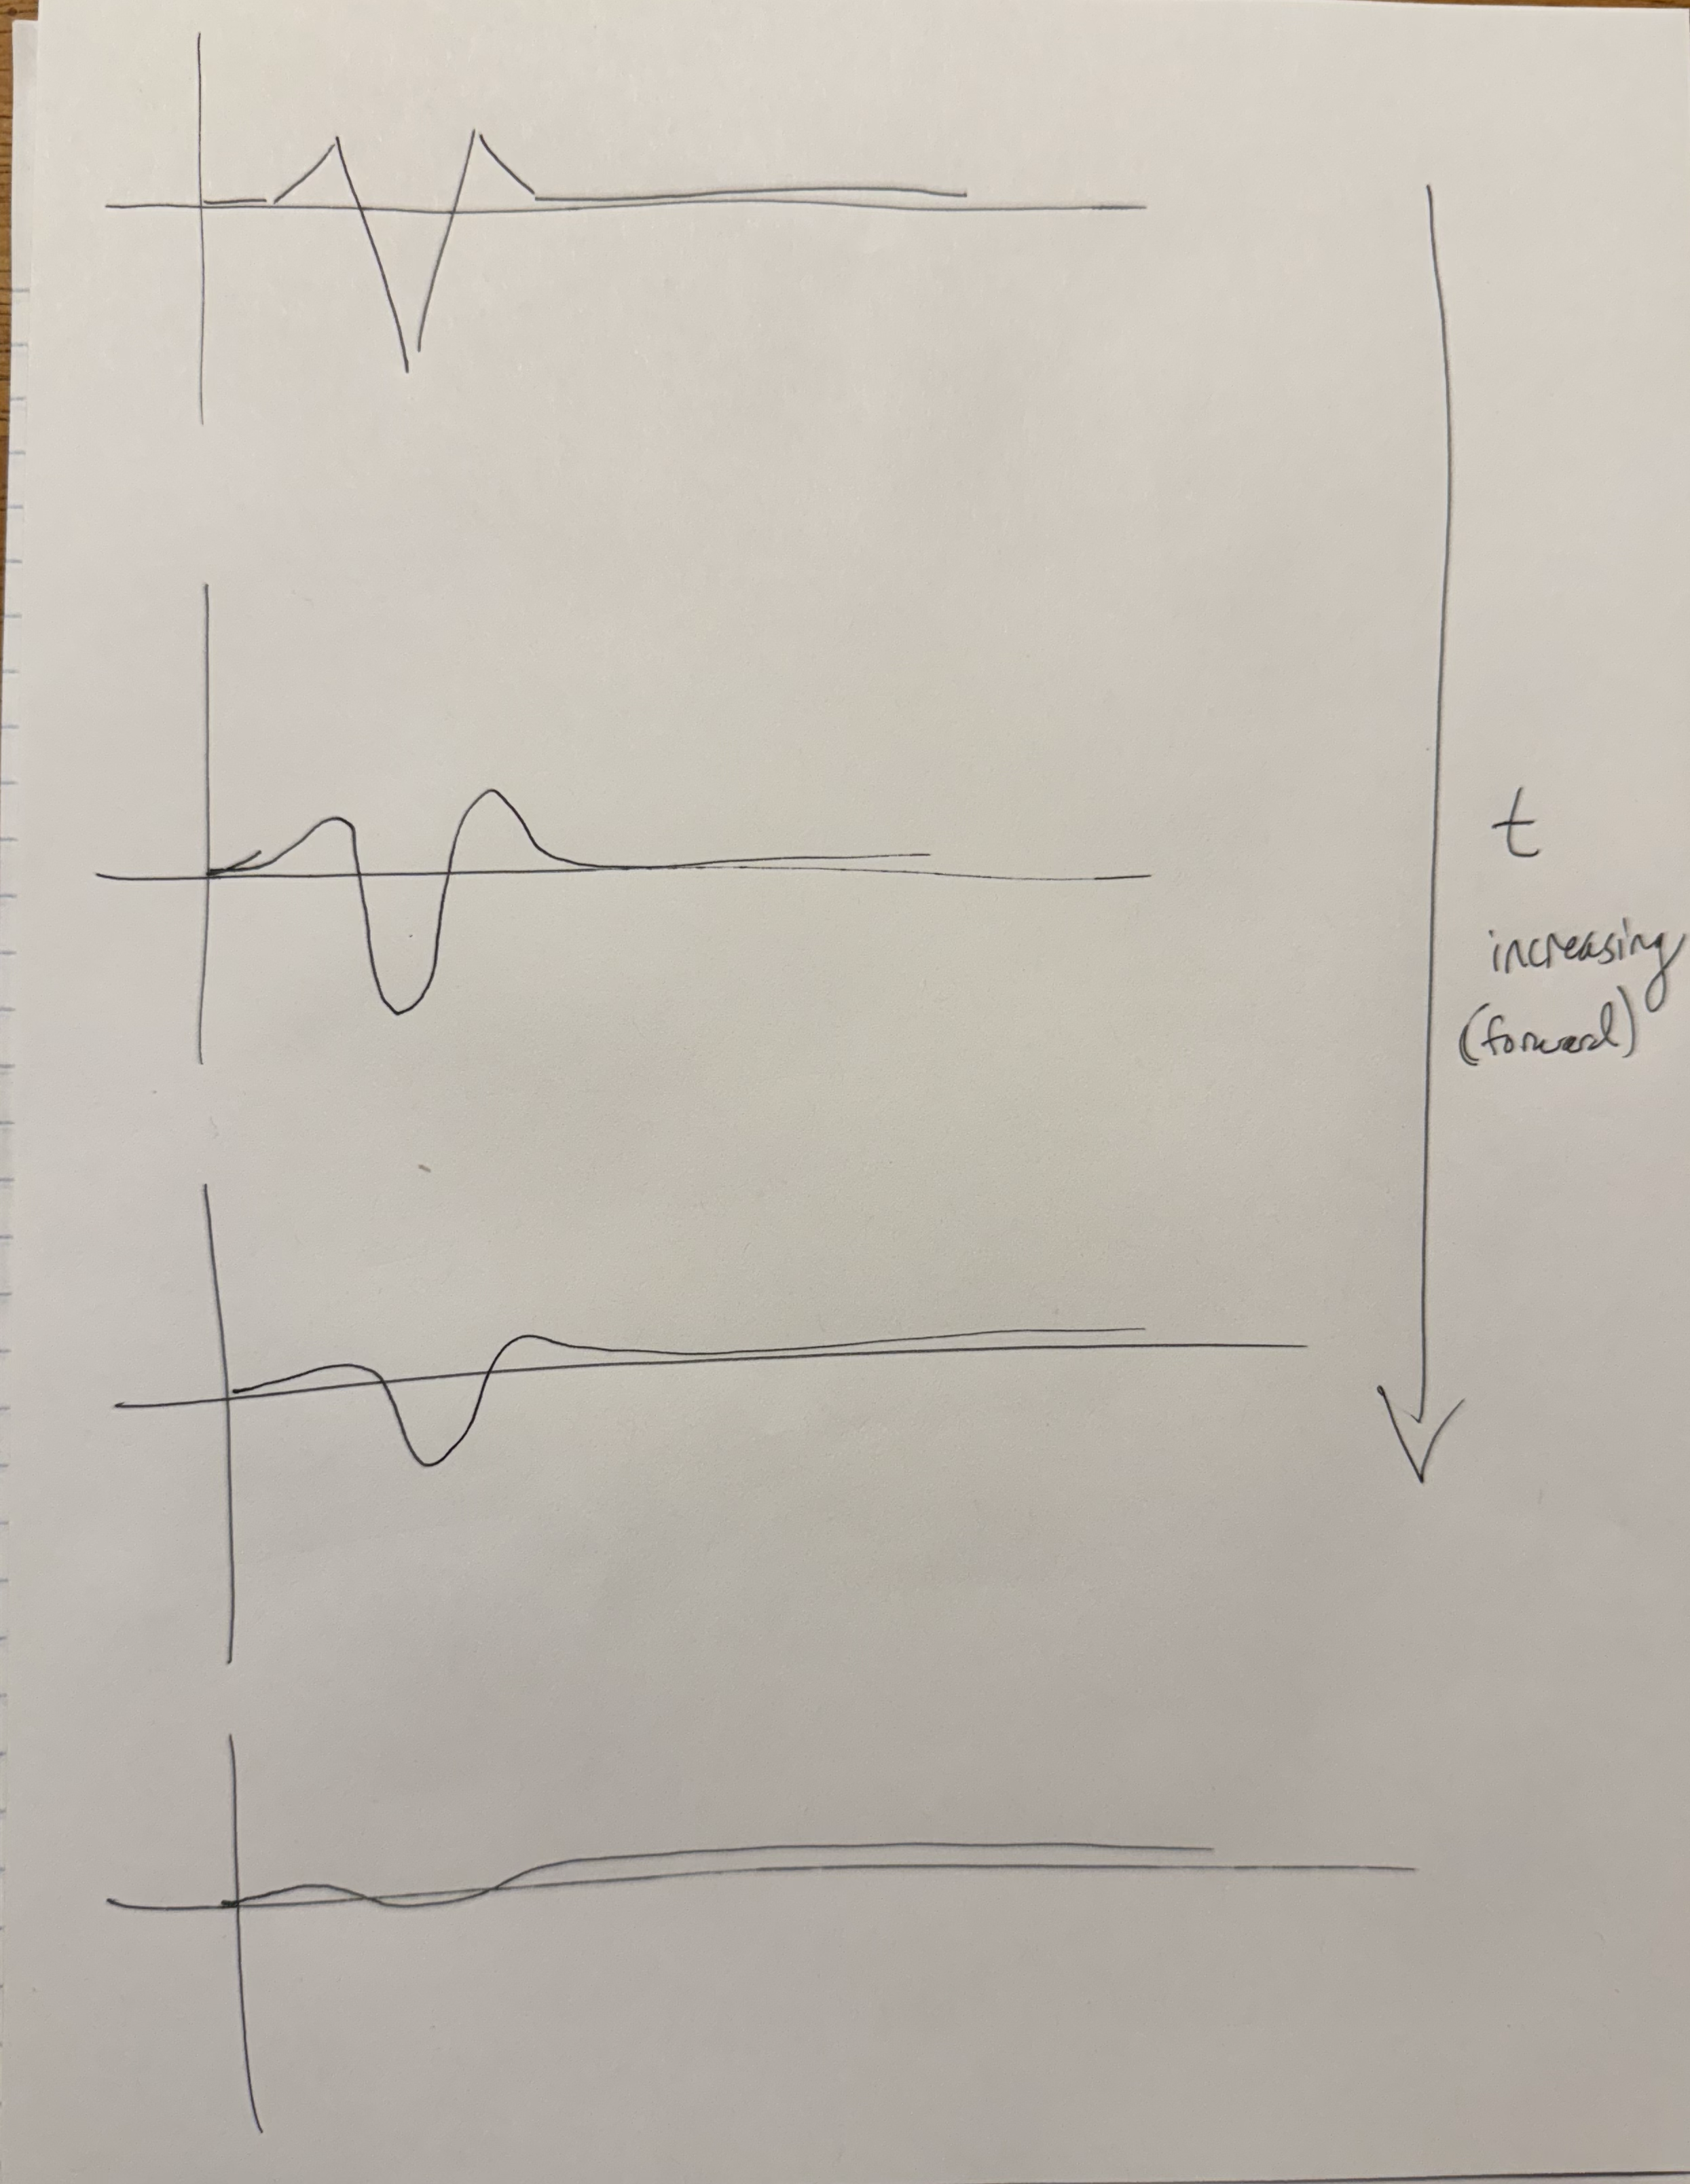
\includegraphics[width=.55\textwidth]{flattening.png}
 	\caption{A sketch of how the curve from problem 1 will evolve over time from the heat equation.}\label{fig:f1}
\end{figure}

\newpage

\item
\begin{enumerate}
\item Consider the following IBVP:
\begin{align*}
\begin{cases}
u_t = u_{xx} + 2, &x \in (0, 1), t > 0 \\
u(0, t) = u(1, t) = 0, & t > 0 \\
u(x, 0) = \E^{x}, &x \in (0, 1)
\end{cases}
\end{align*}
Solve this IBVP in terms of trigonometric series.
Plot the solution $u(x, t)$ at time $t=0$ and $t=100$ by truncating the first 1000 terms of series.
Please describe the behaviors, e.g. discontinuity, smoothness, of the approximate solution when $t=0$ and $t=100$.
In addition, truncate the sin-trigonometric expansion of the function, 2,  by using the first 1000 terms and plot the approximation.
Also, describe the discontinuity and smoothness of the approximate series.

(Hint: try to expand 2 in terms of sin-trigonometric functions at first and the coefficients are determined by the inner product.) \\

\noindent
\textit{Solution:} \\
We begin by finding the sin-trigonometric expansion of 2: \\

\noindent
We have that
$$
2 = \sum_{n=1}^{\infty}d_n \sin(n\pi x)
$$
with each $d_n$ given by
\begin{align*}
d_n &= 2 \int_0^1 2 \sin(n \pi x) dx \\
	&= 4 \left. \left[ -\frac 1 {n \pi} \cos(n \pi x) \right] \right|_0^1 \\
	&= \begin{cases}
	\frac 8 {n \pi}, \quad \text{ when $n$ is odd} \\
	0, \quad \text{ when $n$ is even}.
	\end{cases}
\end{align*}

Next, we assyme $u(x, t) = \sum_{n = 1}^\infty c_n(t) \sin(n\pi x) \E^{- \lambda_n t}$, with $\lambda_n = (n\pi)^2$, from our boundary conditions and heat equation.
So,
\begin{align*}
u_t &= \sum_{n=1}^\infty c_n^\prime(t) \sin(n\pi x) \E^{-\lambda_n t} - \lambda_n c_n(t) \sin(n \pi x)\E^{-\lambda_n t} \\
	&= \sum_{n=1}^\infty \sin(n\pi x) \E^{-\lambda_n t} \left[ c_n^\prime(t) - \lambda_n c_n(t) \right]
\end{align*}
and we also have
$$
u_{xx} = \sum_{n = 1}^\infty \lambda_n c_n(t) \sin(n \pi x) \E^{-\lambda_n t}.
$$
Using $u_t = u_{xx} + 2$, we get
\begin{align*}
c_n^\prime(t)\E^{-\lambda_n t} &= d_n \\
c_n^\prime(t) &= d_n\E^{\lambda_n t} \\
c_n(t) &= \int d_n\E^{\lambda_n t} dt \\
	&=  \frac {d_n} {\lambda_n} \E^{\lambda_n t} + b_n \\
	&=  a_n \E^{\lambda_n t} + b_n
\end{align*}
where $a_n = 8/(n \pi)^3$ when $n$ is odd and 0 when it is even.
This gives us
$$
u(x, t) = \left( \sum_{n = 1}^\infty a_n \sin(n \pi x) \right) + \left( \sum_{n = 1}^\infty b_n \sin(n \pi x) \E^{- \lambda_n t} \right)
$$
with the $b_n$ given from the initial conditions. \\

\noindent
Using $u(x, t) = \E^x$ for $x \in (0, 1)$ and $u(0, t) = u(1, t) = 0$, we write
$$
u(x, 0) = \sum_{n = 1}^\infty \sin(n \pi x) 2 \int_0^1 \E^x \sin(n \pi x) dx
$$
using the sin-trig expansion.
So, 
$$
a_n + b_n = 2 \int_0^1 \E^x \sin(n \pi x) dx.
$$
Let $I_n = \int_0^1\E^x \sin(n \pi x) dx$.
Solving this yields, 
$$
u = \sin(n \pi x), \quad v = \E^x, \quad du = n \pi \cos (n \pi x), \quad dv = \E^x
$$
then
$$
I_n = \E^x\sin(n \pi x) - n \pi \int_0^1\E^x \cos(n \pi x) dx.
$$
Repeating we have
$$
u = \cos(n \pi x), \quad v = \E^x, \quad du = - n \pi \sin (n \pi x), \quad dv = \E^x
$$
giving us
\begin{align*}
I_n &= -n \pi \left[ \E^x \cos(n \pi x)|_0^1 + n \pi I_n \right] \\
I_n (1 + (n \pi)^2) &= n \pi (1 - (-1)^n\E) \\
I_n &= \frac{n \pi (1 - (-1)^n\E)}{1 + (n \pi)^2}.
\end{align*}
So, $b_n = 2I_n - a_n$.

Therefore, we have found u:
$$
u(x, t) = \sum_{n = 1}^\infty \left[a_n + b_n \E^{-(n \pi)^2 t} \right] \sin (n \pi x), 
$$
with $a_n$ and $b_n$ defined as above. \\
\qed

\newpage


\item Consider the following IBVP:
\begin{align*}
\begin{cases}
u_t = u_{xx} + \cos 2x, &x \in (0, \pi), t > 0 \\
u_x(0, t) = u_x(\pi, t) = 0, & t > 0 \\
u(x, 0) = x^2(\pi - x)^2, &x \in (0, \pi)
\end{cases}
\end{align*}
Solve this IBVP in terms of trigonometric series.
Plot the solution $u(x, t)$ at time $t=0$ and $t=100$ by truncating the first 1000 terms of series.
Please describe the behaviors, e.g. discontinuity, smoothness, of the approximate solution when $t=0$ and $t=100$. \\

\noindent
\textit{Solution:} \\
\textbf{TODO} \\

\end{enumerate}

\newpage

\item
\begin{enumerate}
\item Consider the following IBVP:
\begin{align*}
\begin{cases}
u_t = u_{xx}, &x \in (0, \pi), t > 0 \\
u(0, t) = 0, \: u(\pi, t) = \pi, & t > 0 \\
u(x, 0) = \frac 1 2 \sin x + x, &x \in (0, \pi)
\end{cases}
\end{align*}
Solve this IBVP to get the general solution. \\

\noindent
\textit{Solution:} \\
Let $w(x)$ be the stationary distribution of the heat equation.
We solve to find:
$$
w_t = 0 \implies w_{xx} = 0 \implies w(x) = c_1x + c_2.
$$
Using our boundary conditions: $w(x) = x$.
Let $u(x, t) = v(x, t) + w(x)$, then at $t=0$, we have
$$
v(x, 0) = \frac 1 2 \sin x.
$$
From $u_t = u_xx$ we get
$$
v_t + w_t = v_{xx} + w_{xx}.
$$
Thus, $v_t = v_{xx}$.
With $v = u - w$, we get the boundary conditions $v(0, t) = v(\pi, t) = 0$.
From the heat equation we know
$ v(x, t) = \frac 1 2 \sin(x) \E^{-t}. $
Hence, $u(x, t) = \frac 1 2 \sin(x)\E^{-t} + x. $ \\
\qed \\

\item Consider the following IBVP:
\begin{align*}
\begin{cases}
u_t = u_{xx}, &x \in (0, \pi), t > 0 \\
u_x(0, t) = 1, \quad u_x(\pi, t) = \frac 3 4, & t > 0 \\
u(x, 0) = \frac 1 2 \cos \left( \frac x 2 \right) + x, &x \in (0, \pi)
\end{cases}
\end{align*}
Introduce an intermediate function $w$ to eliminate inhomogeneous NBC and transform the problem into IBVP with homogeneous NBC and inhomogeneous source. \\

\noindent
\textit{Solution:} \\
We find a distribution $w$ to homogenize the Neumann boundary condition (NBC)
\begin{align*}
w(x) &= c_1x^2 + c_2x, \\
w_x &= 2c_1x + c_2, \quad w_x(0) = 1 \text{ and } w_x(\pi) = 3/4 \\
&\implies w(x) = x- \frac 1 {8 \pi}x^2
\end{align*}
Let $u(x, t) = w(x) + v(x, t)$.
So, 
$$
v(x, t) = u(x, t) - w(x) \implies v(x, 0) = \frac 1 2 \cos (x/2) + \frac 1 {8 \pi} x^2
$$
and $u_t = u_{xx} \implies v_t = -\frac 1 {4 \pi} + v_{xx}$ with $v_x(0, t) = v_x(\pi, t) = 0$.
Therefore, we have transformed the IBVP into the one with homogenous NBC and the inhomogeneous source, where
$$
u(x, t) = v(x, t) + x - \frac 1 {8 \pi}x^2.
$$
\qed \\

\end{enumerate}

\newpage

\item Olver 4.1.4. Find a series solution to the initial-boundary value problem for the heat equation $u_t = u_{xx}$ for $0 < x < 1$ when one the end of the bar is held at 0\textdegree \, and the other is insulated.
Discuss the asymptotic behavior of the solution as $t \rightarrow \infty$. \\

\noindent
\textit{Solution:} \\
Note the important information here is that $x \in [0, 1]$, $u(0, t) = 0$ and $u_x(1, t) = 0$ and we are assuming $u(x, 0) = f(x)$.
We begin by assuming $u(x, t) = X(x)T(t)$, plugging this into the PDE we have
$$
T^\prime X = X^{\prime\prime}T.
$$
Similar to HW 1 we then have
$$
\frac {T^\prime}T = \frac {X^{\prime\prime}} X = -\lambda
$$
Therefore we need to solve the following
\begin{align*}
T^\prime + \lambda T &= 0, \\
X^{\prime\prime} + \lambda X &= 0, \quad X(0) = 0, \: X^\prime(1) = 0.
\end{align*}
First, we solve for $X$. \\

\noindent
\underline{Case 1 $\lambda < 0$:} \\
Let $-\lambda = h^2$ then we have
$$
X(x) = A \cosh (hx) + B \sinh (hx)
$$
This implies that $X(0) = A = 0$ and thus $X(x) = B\sinh(hx)$.
Therefore,  $X^\prime(x) = hB\cosh(hx)$ and thus we need
$$
X^\prime(1) = hB\cosh(h) = 0
$$
which is not possible so this case does not provide us with our solution. \\

\noindent
\underline{Case 2 $\lambda = 0$:} \\
Then we have $X(x) = Ax + B$.
Using the initial condition $X(0) = 0$ we then conclude that $X(x) = Ax$.
Next, $X^\prime(1) = 0$ implies that $A = 0$ and thus this is just the trivial case and is not our solution. \\

\noindent
\underline{Case 3 $\lambda > 0$:} \\
Then we have $X(x) = A\cos (\sqrt \lambda x) + B\sin (\sqrt \lambda x)$.
Using the initial condition $X(0) = 0$ we then conclude that $X(0) = A = 0$.
Thus we have $X(x) = B\sin(\sqrt \lambda x)$.
Now the other condition $X^\prime(1) = \sqrt \lambda B \cos(\sqrt \lambda) = 0$.
This will only happen if $\cos(\sqrt \lambda) = 0$ which implies that $\sqrt \lambda = k\pi/2$ for an odd integer $k$.
Thus we have the collection of solutions
$$
\lambda_k = \left(\frac {k \pi} 2 \right)^2, \quad X_k = \sin \left( \frac {k \pi x}{2}\right), \quad \text{for}\: k = 1, 3, 5, ....
$$
Next we solve for $T$, from HW 1 we can jump to the following
$$
T_k(t) = b_k\E^{- \left( \frac {k \pi} 2 \right)^2 t}
$$
where $b_k$ comes from initial conditions. \\

\noindent
Since $u_k(x, t) = X_k(x)T_k(t)$, then we have
$$
u(x, t) = \sum_{k = 1}^\infty b_{2k - 1}\E^{- \left( \frac {(2k - 1) \pi} 2 \right)^2 t}\sin \left( \frac {(2k - 1) \pi x}{2}\right).
$$
To calculate the $b_k$ terms we use the initial condition that $u(x, 0) = f(x), x\in (0, 1)$, this gives
\begin{align*}
f(x) &= \sum_{k = 1}^\infty b_{2k - 1}\E^{- \left( \frac {(2k - 1) \pi} 2 \right)^2 0}\sin \left( \frac {(2k - 1) \pi x}{2}\right) \\
f(x) &= \sum_{k = 1}^\infty b_{2k - 1}\sin \left( \frac {(2k - 1) \pi x}{2}\right) \\
f(x)\sin \left( \frac {m \pi x}{2}\right) &= \sum_{k = 1}^\infty b_{2k - 1}\sin \left( \frac {(2k - 1) \pi x}{2}\right)\sin \left( \frac {m \pi x}{2}\right) \\
\int_0^1 f(x)\sin \left( \frac {m \pi x}{2}\right) dx &= \int_0^1 \sum_{k = 1}^\infty b_{2k - 1}\sin \left( \frac {(2k - 1) \pi x}{2}\right)\sin \left( \frac {m \pi x}{2}\right) dx
\end{align*}
We can obviously now see that the
$$b_k = 2 \int_0^1 f(x) \sin \left(\frac {k \pi x} 2\right) dx.$$
Therefore, finally, 
$$
u(x, t) = \sum_{k = 1}^\infty \left[ 2 \int_0^1 f(x) \sin \left(\frac {(2k - 1) \pi x} 2\right) dx \right]\E^{- \left( \frac {(2k - 1) \pi} 2 \right)^2 t}\sin \left( \frac {(2k - 1) \pi x}{2}\right).
$$
For the asymptotic long term behavior as $t\rightarrow \infty$ the exponential term goes to 0 and thus the whole expression goes to 0 at an exponential rate.
Since one end of the rod is held at 0 degrees then the whole rod will eventually settle to 0 degrees.
Since the other end of the rod is insulated (by our boundary condition) we know that the heat will be lost through other parts of the rod. \\
\qed \\

\newpage

\item Olver 3.2.2 Find the Fourier series of the following functions:
\begin{enumerate}

\item Problem (b):
$$
\begin{cases}
1, &\frac 1 2 \pi < |x| < \pi \\
0, &\text{otherwise}
\end{cases}
$$ \\

\noindent
\textit{Solution:} \\
Again, we want to find the formula for the following given our function $f$,
$$
f(x) \sim \frac {a_0} 2 + \sum_{k = 1}^\infty \left[ a_k \cos kx + b_k \sin kx \right]
$$
where the coefficients are given by
\begin{align*}
a_k = \langle f, \cos kx \rangle = \frac 1 \pi \int_{-\pi}^\pi f(x) \cos kx dx, \quad &k = 0, 1, 2, 3, ..., \\
b_k = \langle f, \sin kx \rangle = \frac 1 \pi \int_{-\pi}^\pi f(x) \sin kx dx, \quad &k = 1, 2, 3, ....
\end{align*}
Notice, our function, $f$ is an even function, therefore the $b_k$ coefficients of the $\sin kx$ term will be zero since $\sin$ is odd and there is no need for odd contributions to this function, $f$.
Therefore we need only solve for the $a_k$'s.
Beginning by splitting up the integral into the portions of the piecewise nature of $f$ on the interval $[-\pi,\pi]$.
First, however, notice for $k = 0$ the antiderivative of our integrand will be undefined so we treat that case separately later.
For $k > 0$ we have
\begin{align*}
a_k = \langle f, \cos kx \rangle &= \frac 1 \pi \int_{-\pi}^\pi f(x) \cos kx dx \\
	&= \frac 1 \pi \left[ \int_{-\pi}^{-\pi/2} \cos kx dx +  \int_{\pi/2}^{\pi} \cos kx dx \right] \\
	&= \frac 1 \pi \left[ \left. \frac 1 k \sin kx \right|_{-\pi}^{-\pi/2} + \left. \frac 1 k \sin kx \right|_{\pi/2}^{\pi} \right] \\
	&= \frac 1 \pi \left[ \frac 1 k \big( \sin (-k\pi/2) - \sin (- k\pi) \big) + \frac 1 k \big( \sin (k \pi) - \sin (k\pi/2) \big) \right] \\
	&= \frac 1 {k\pi} \Big[ \sin (-k\pi/2) - \sin (- k\pi) + \sin (k \pi) - \sin (k\pi/2) \Big].
\end{align*}
We can further simplify using our understanding that $\sin$ is an odd function thus $\sin(-\theta) = -\sin\theta$
\begin{align*}
a_k &= \frac 1 {k\pi} \Big[ - \sin (k\pi/2) + \sin (k\pi) + \sin (k \pi) - \sin (k\pi/2) \Big] \\
	&= \frac 1 {k\pi} \Big[ - 2 \sin (k\pi/2) + 2 \sin (k\pi) \Big] \\
	&= \frac 2 {k\pi} \Big[ \cancelto{0}{\sin (k\pi)} - \sin (k\pi/2) \Big] \\
	&= - \frac 2 {k\pi} \sin (k\pi/2).
\end{align*}
Finally in the case that $k = 0$ we have
\begin{align*}
a_0 = \langle f, \cos 0 \rangle = \frac 1 \pi \int_{-\pi}^\pi f(x) \cos (0x) dx &= \frac 1 \pi \int_{-\pi}^\pi f(x) dx \\
	&= \frac 1 \pi \left[ \int_{-\pi}^{-\pi/2} dx +  \int_{\pi/2}^{\pi} dx \right] \\
	&= \frac 1 \pi \Big[ -\pi/2 - (-\pi) + \pi - \pi/2 \Big] \\
	&= \frac 1 \pi \Big[ -\pi/2 + \pi + \pi - \pi/2 \Big] = 1.
\end{align*}
Therefore we have the Fourier series for the piecewise function $f$ as
$$
f(x) \sim f(x) \sim \frac 1 2 - \sum_{k = 1}^\infty \frac 2 {k\pi} \sin (k\pi/2) \cos kx
$$

\item Problem (e)
$$
\begin{cases}
\cos x, & |x| < \frac 1 2 \pi \\
0, &\text{otherwise}
\end{cases}
$$ \\

\noindent
\textit{Solution:} \\
Once again the meat of our work comes down to calculating the coefficients $a_k$ and $b_k$.
Once again, since our function $f$ is even we can ignore the $b_k$ terms.
Now as we calculate the $a_k$ terms let's consider several cases.
First we have
\begin{align*}
a_k = \langle \cos x, \cos kx \rangle = \frac 1 \pi \int_{-\pi}^\pi f(x) \cos kx dx
	&= \frac 1 \pi \int_{-\pi/2}^{\pi/2} \cos x \cos kx dx \\
	&= \frac 1 {2\pi} \int_{-\pi/2}^{\pi/2} \Big[ \cos ((1+ k)x) + \cos ((1- k)x) \Big]dx \\
\end{align*}
Now when $k = 0$ we have the following
\begin{align*}
a_0 = \frac 1 {2\pi} \int_{-\pi/2}^{\pi/2} \Big[ \cos ((1+ 0)x) + \cos ((1- 0)x) \Big]dx &= \frac 1 {2\pi} \int_{-\pi/2}^{\pi/2} 2\cos x dx \\
	&= \frac 1 \pi \left. \sin x \right|_{-\pi/2}^{\pi/2} \\
	&= \frac 1 \pi \Big( \sin (\pi/2) - \sin (- \pi/2) \Big) \\
	&= \frac 1 \pi \Big( 1 - (-1) \Big) = \frac 2 \pi.
\end{align*}
Then when $k = 1$ we have
\begin{align*}
a_1 = \frac 1 {2\pi} \int_{-\pi/2}^{\pi/2} \Big[ \cos ((1+ 1)x) + \cos ((1- 1)x) \Big]dx &= \frac 1 {2\pi} \int_{-\pi/2}^{\pi/2} \cos 2x + 1dx \\
	&= \frac 1 {2\pi} \left[ \left. \frac 1 2 \sin 2x + x\right|_{-\pi/2}^{\pi/2} \right] \\
	&= \frac 1 {2\pi} \left[ \frac 1 2 \sin (\pi/2) + \pi/2 - \frac 1 2 \sin (- \pi/2) - (-\pi/2) \right] \\
	&= \frac 1 {2\pi} \left[ \sin (\pi/2) + \pi \right] \\
	&= \frac 1 {2\pi} \left[ 1 + \pi \right].
\end{align*}

\textbf{TODO: Come back to solve for the generic $k$ case.}

\end{enumerate}
\newpage

\item Olver 3.2.3 Find the Fourier series of $\sin^2 x$ and $\cos^2 x$ without directly calculating the Fourier coefficients.
Hint: Use some standard trigonometric identities.\\

\noindent
\textit{Solution:} \\
For my personal reference throughout this assignment here is the version of the Fourier Series that we are using in this course.
For a function $f(x)$ defined on $-\pi \leq x \leq \pi$ is
$$
f(x) \sim \frac {a_0} 2 + \sum_{k = 1}^\infty \left[ a_k \cos kx + b_k \sin kx \right]
$$
where the coefficients are given by
\begin{align*}
a_k = \langle f, \cos kx \rangle = \frac 1 \pi \int_{-\pi}^\pi f(x) \cos kx dx, \quad &k = 0, 1, 2, 3, ..., \\
b_k = \langle f, \sin kx \rangle = \frac 1 \pi \int_{-\pi}^\pi f(x) \sin kx dx, \quad &k = 1, 2, 3, ....
\end{align*}
Now for this problem, we want to avoid calculating manually the Fourier coefficients, but instead use a common trig identity.
For $\sin^2 x$, recall
$$
\sin^2 x = \frac {1 - \cos 2x} 2 = \frac 1 2 - \frac 1 2 \cos 2x.
$$
Which happens to be in the form of the Fourier series where $a_0 = 1, a_1 = 0, a_2 = -1/2$ while the rest of the $a_k$'s and all $b_k$'s are 0.
Similarly we have
$$
\cos^2 x = \frac {1 + \cos 2x} 2 = \frac 1 2 + \frac 1 2 \cos 2x.
$$
for $\cos^2 x$ from the common trig identity. \\
\qed \\

\newpage

\item Olver P73, Lemma 3.1 in Olver.
To obtain full credits, please give the detailed calculation of the integrals and show how to use trigonometric identities or integration by parts (if used) step by step. \\

\noindent
As stated in the text \\
\textit{Lemma 3.1}: Under the rescaled $L^2$ inner product, the trigonometric functions $1, \sin x, \cos x, \sin 2 x, \cos 2x , ..., $ satisfy the following orthogonality relations:
\begin{align*}
\langle \cos k x, \cos \ell x \rangle = \langle \sin k x, \sin \ell x \rangle = 0, \quad &\text{for}\: k \neq \ell \\
\langle \cos k x, \sin \ell x \rangle = 0, \quad  &\text{for all}\: k, \ell \\
||1|| = \sqrt 2, \quad || \cos k x || = || \sin k x || = 0,  \quad &\text{for}\: k \neq 0
\end{align*}
where $k, \ell$ are nonnegative integers. \\

\noindent
\textit{Solution:} Now we are being asked to show the detailed calculations of the various integrals as presented in the text to prove this lemma.
We first calculate
\begin{align*}
\int_{-\pi}^{\pi} \cos kx \cos l x dx
	&= \frac 1 2 \int_{-\pi}^{\pi} \cos \big( (k + l) x\big) + \cos \big( (k - l) x\big) dx \\
\end{align*}
Assume $k = l \neq 0$ then we have
\begin{align*}
\frac 1 2 \int_{-\pi}^{\pi} \cos \big( (k + l) x\big) + \cos \big( (k - l) x\big) dx 
	&= \frac 1 2 \int_{-\pi}^{\pi} \cos \big( 2k x\big) + 1 dx \\
	&= \frac 1 2 \int_{-\pi}^{\pi} \cos \big( 2k x\big) dx + \frac 1 2 \int_{-\pi}^{\pi} dx \\
	&= \cancelto{0}{\frac 1 2 \left( \frac 1 {2k} \sin\big( 2k \pi\big) - \frac 1 {2k} \sin\big( - 2k \pi\big) \right) }+ \frac 1 2( \pi - (-\pi) )
	&= \pi.
\end{align*}
Alternatively, if $k = l = 0$, then from the beginning we only have
\begin{align*}
\int_{-\pi}^{\pi} \cos kx \cos l x dx = \int_{-\pi}^{\pi} \cos 0x \cos 0 x dx = \int_{-\pi}^{\pi} dx = \pi - (-\pi) = 2\pi.
\end{align*}
Finally, when $k \neq l$ we have
\begin{align*}
\int_{-\pi}^{\pi} \cos kx \cos l x dx
	&= \frac 1 2 \Bigg[ \cancelto{0}{\int_{-\pi}^{\pi} \cos \big( (k + l) x\big)dx} + \cancelto{0}{\int_{-\pi}^{\pi} \cos \big( (k - l) x\big) dx} \Bigg] = 0 \\
\end{align*}
Where each of these $\cos$ integrals are equal to 0 due to the fact that they are even functions integrating across an interval centered at 0. \\

\noindent
Next, we need to calculate the following for the two cases $k \neq l$ and $k = l \neq 0$
\begin{align*}
\int_{-\pi}^{\pi} \sin kx \sin l x dx
	&= \frac 1 2 \Bigg[ \int_{-\pi}^{\pi} \cos \big( (k - l) x\big)dx - \int_{-\pi}^{\pi} \cos \big( (k + l) x\big) dx \Bigg] \\
\end{align*}
When $k \neq l$ we have
\begin{align*}
\frac 1 2 \Bigg[ \cancelto{0}{\int_{-\pi}^{\pi} \cos \big( (k - l) x\big)dx} - \cancelto{0}{\int_{-\pi}^{\pi} \cos \big( (k + l) x\big) dx} \Bigg] \\
\end{align*}
for the same reasons as before with $\cos$ and the interval centered at 0.
Once more, when $k = l \neq 0$ we have
\begin{align*}
\int_{-\pi}^{\pi} \sin kx \sin l x dx
	&= \frac 1 2 \Bigg[ \int_{-\pi}^{\pi} dx - \cancelto{0}{\int_{-\pi}^{\pi} \cos \big( (k + l) x\big) dx} \Bigg] \\
	&= \frac 1 2 \Bigg[ \pi - (-\pi) \Bigg] \\
	&= \pi.
\end{align*}

\noindent
Finally, we want to calculate
$$
\int_{-\pi}^{\pi} \cos kx \sin l x dx.
$$
Notice, the product of an even and an odd function is an odd function.
Additionally recall that integrating an odd function over an interval symmetric about 0, the result is 0.
Thus
$$
\int_{-\pi}^{\pi} \cos kx \sin l x dx = 0, \quad \forall k, l \in \mathbb Z.
$$
\qed \\
\end{enumerate}

\end{document}

%%% Local Variables:
%%% mode: latex
%%% TeX-master: t
%%% End:
